\documentclass[english, paper=a4]{scrartcl}
\usepackage[utf8]{inputenc}
% images
\usepackage{graphicx}
%math
\usepackage{amsmath,amssymb}
%code
\usepackage{algorithm}
\usepackage[noend]{algpseudocode}
\makeatletter
\def\BState{\State\hskip-\ALG@thistlm}
\makeatother

\usepackage{subcaption}
\captionsetup{compatibility=false}
\usepackage{multirow}
\usepackage{color}
\usepackage{enumitem}


\begin{document}

\graphicspath{{images/}}

%%------------------------------------------------------
\title{Local Stereo Matching using OpenCV\\Part 2: Disparity Selection based on Absolute Intensity Difference Cost Volume} 
\subtitle{Stereo Vision 2017S, TU Vienna} 
\author{Johanna Donabauer (), Nikolaus Leopold (1327344)}
\maketitle
%%------------------------------------------------------

\section{Evaluation using Middlebury Dataset}

\begin{figure}[H]
\centering
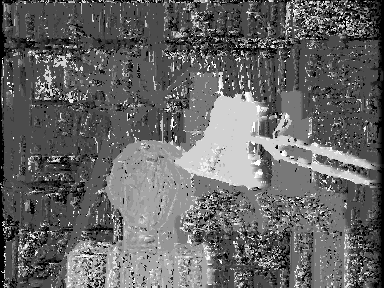
\includegraphics[width=0.49\textwidth]{tsukuba_result_left_winsize3_mindisp15.png}
\label{fig:tsukuba_result_left_winsize3_mindisp15}
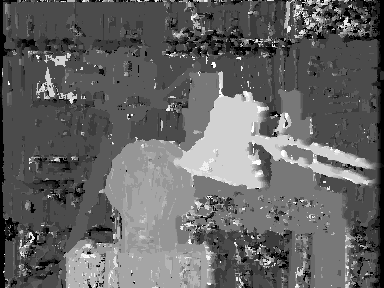
\includegraphics[width=0.49\textwidth]{tsukuba_result_left_winsize5_mindisp15.png}
\label{fig:tsukuba_result_left_winsize5_mindisp15}
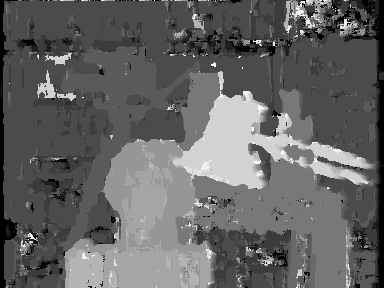
\includegraphics[width=0.49\textwidth]{tsukuba_result_left_winsize7_mindisp15.png}
\label{fig:tsukuba_result_left_winsize7_mindisp15}
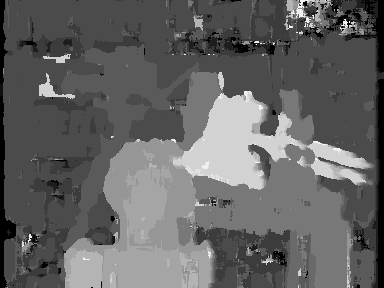
\includegraphics[width=0.49\textwidth]{tsukuba_result_left_winsize9_mindisp15.png}
\label{fig:tsukuba_result_left_winsize9_mindisp15}
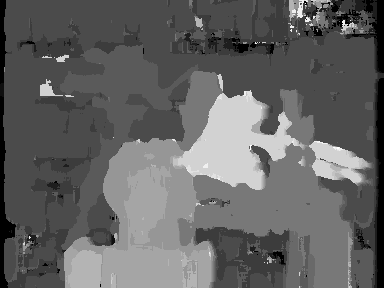
\includegraphics[width=0.49\textwidth]{tsukuba_result_left_winsize11_mindisp15.png}
\label{fig:tsukuba_result_left_winsize11_mindisp15}
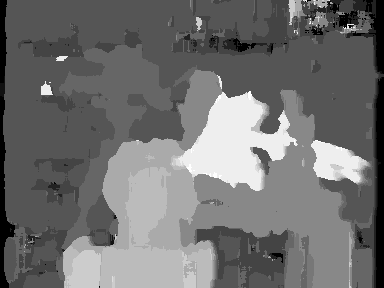
\includegraphics[width=0.49\textwidth]{tsukuba_result_left_winsize13_mindisp15.png}
\label{fig:tsukuba_result_left_winsize13_mindisp15}
\caption{Resulting left disparity maps for the \texttt{tsukuba} image pair from the 2001 Middlebury stereo vision dataset, using \texttt{minDisparity}~15 and \texttt{windowSize} 3, 5, 7, 9, 11, 13 from top-left to bottom-right. 7 or 9 may be assumed the best window size for this image pair, as a compromise between noise and loss of connectivity of fine detail.}
\end{figure}

\begin{figure}[H]
\centering
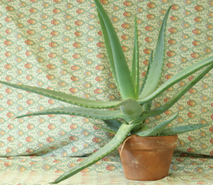
\includegraphics[width=0.49\textwidth]{aloe_left.png}
\label{fig:aloe_left}
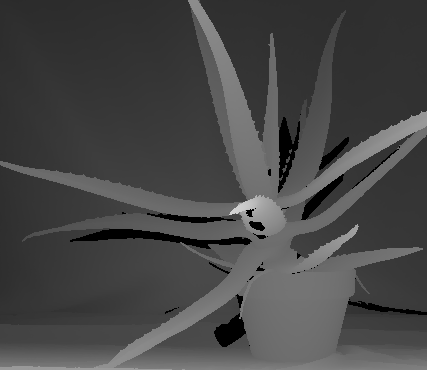
\includegraphics[width=0.49\textwidth]{aloe_groundtruth_left.png}
\label{fig:aloe_groundtruth_left}
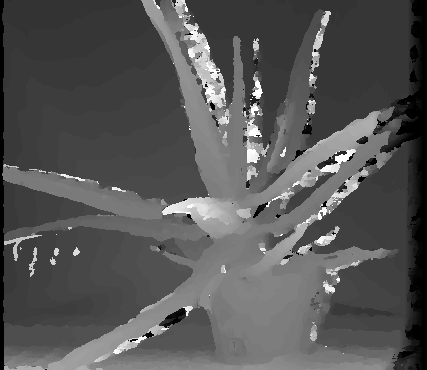
\includegraphics[width=0.49\textwidth]{aloe_result_left_winsize9_mindisp75.png}
\label{fig:aloe_result_left_winsize9_mindisp75}
\caption{Top: Left image and left disparity map ground truth of the \texttt{aloe} image pair from the 2006 Middlebury stereo vision dataset.\\
Bottom: Resulting left disparity map, using \texttt{minDisparity}~75 and \texttt{windowSize}~9. Note that the background disparity was accurately computed thanks to the textured backdrop.}
\end{figure}

\begin{figure}[H]
\centering
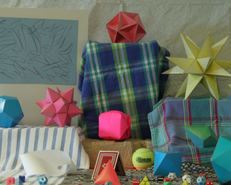
\includegraphics[width=0.49\textwidth]{moebius_left.png}
\label{fig:moebius_left}
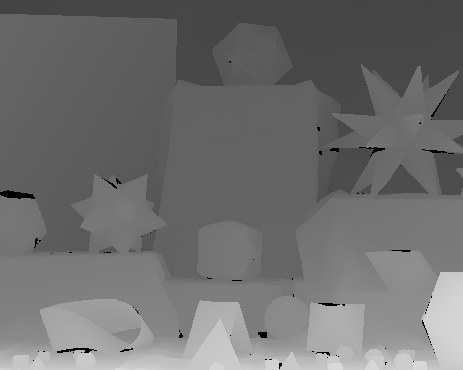
\includegraphics[width=0.49\textwidth]{moebius_groundtruth_left.png}
\label{fig:moebius_groundtruth_left}
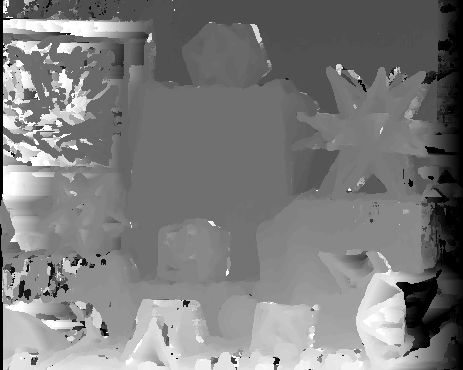
\includegraphics[width=0.49\textwidth]{moebius_result_left_winsize7_mindisp75.png}
\label{fig:moebius_result_left_winsize7_mindisp75}
\caption{Top: Left image and left disparity map ground truth of the \texttt{moebius} image pair from the 2005 Middlebury stereo vision dataset.\\
Bottom: Resulting left disparity map, using \texttt{minDisparity}~75 and \texttt{windowSize}~7. Note the interesting errors in the drawing in the top-left corner. Incorporating spatial difference information additional to the currently used absolute intensity difference in the search windows may yield better results.}
\end{figure}

\begin{figure}[H]
\centering
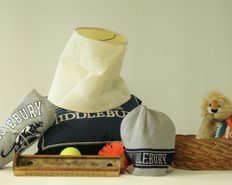
\includegraphics[width=0.49\textwidth]{midd1_left.png}
\label{fig:midd1_left}
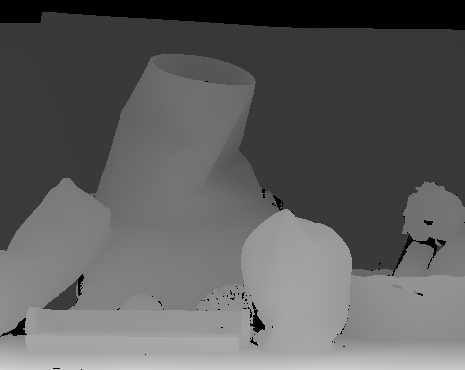
\includegraphics[width=0.49\textwidth]{midd1_groundtruth_left.png}
\label{fig:midd1_groundtruth_left}
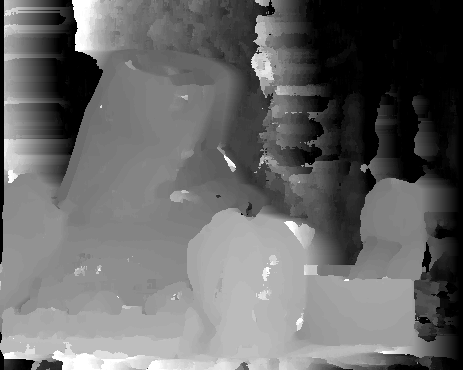
\includegraphics[width=0.49\textwidth]{midd1_result_left_winsize11_mindisp75.png}
\label{fig:midd1_result_left_winsize11_mindisp75}
\caption{Top: Left image and left disparity map ground truth of the \texttt{midd1} image pair from the 2006 Middlebury stereo vision dataset.\\
Bottom: Resulting left disparity map, using \texttt{minDisparity}~75 and \texttt{windowSize}~11. Note the errors in the background due to lack of texture. Incorporating spatial difference information additional to the currently used absolute intensity difference in the search windows may yield better results.}
\end{figure}

%%------------------------------------------------------

\newpage

\bibliographystyle{plain}
\bibliography{lit}
%% References can be stored in a seperate bib-file (see lit.bib). References, that are cited in the report using \cite are automatically added to the reference list. For more information: http://www.bibtex.org/Using/
%%------------------------------------------------------
\end{document}
